\chapter{序論}
\thispagestyle{fancy}
\nobreak
\section{研究背景と目的}
本研究は「オーディトリウムの“底”で演奏を聴く」という旧態依然とした鑑賞形態並びにそれに基づく決定論的設計法に対し、建築音響学の観点から新たな息吹を吹き込むことで、次世代の建築を設計するための礎を築こうとするものである。

\subsection{2階バルコニー最前列席の音響的評価}
この世に存在する全てのオーディトリウムはいずれも室固有の響きを持っており、それは室を構成する形と内装条件によって決定づけられる。一般的な音響設計では、どの客席においても一様な反射音が到達するよう計画される。
ここで、収容人数や舞台へ向けての視野を確保する観点から、オーディトリウムにバルコニー席を設けることが多々ある。このとき、バルコニー先端部は前方に客席がなく、ホール空間へ張り出した特異な場となる。
\\ さて、2階バルコニー最前列の座席は、音響的に高い評価を得ることが多い$^{\text{\cite{01-1}}}$。これは、ホール空間が有する吸音力の大半(500Hzで7割程度)$^{\text{\cite{01-2}}}$を受け持っている1階客席床面(椅子+聴衆の吸音力)から相対的に離れた場所に位置するため、エネルギ減衰の少ない有効な直接音や反射音を得やすいことに起因すると定性的に推察されている(\textgt{図}\ref{fig:2階バルコニー最前列席の音場})。
\\
\\
\begin{figure}[h]
    \centering
    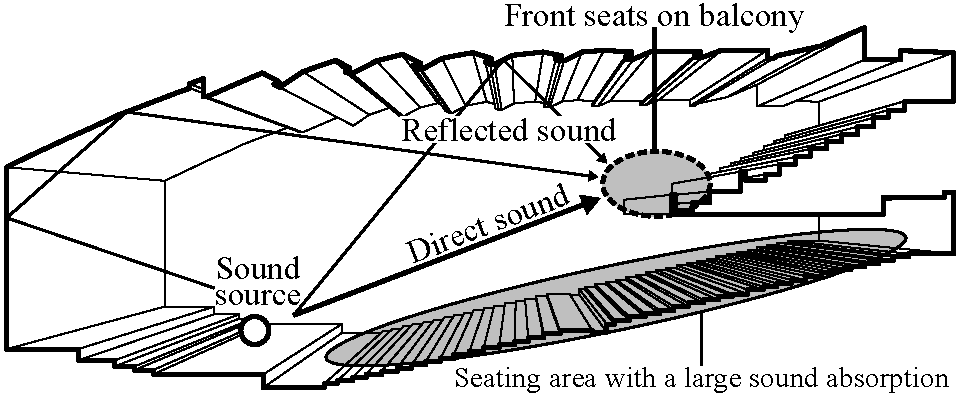
\includegraphics[keepaspectratio,scale=0.8]{01_att/second_balcony.pdf}
    \caption{\hspace{1mm}2階バルコニー最前列席の音場}
    \label{fig:2階バルコニー最前列席の音場}
\end{figure}

%-------------------------------------------------------------
\newpage
\subsection{評価対象領域の拡張}
美しい響きを生み出すにあたり、室容積は人間を収容するには冗長な大きさを要する。規模により異なるものの、室容積から算出されるホールの天井高はおおよそ10$\sim$20mである。ホール空間は人が鑑賞可能なエリアを断面方向含め無数に拡張できるというポテンシャルを秘めているにも関わらず、オーディトリウムの底で鑑賞をするという様式は依然として変わっていない。
\\ 建築音響学が体系化した1900年以後$^{\text{\cite{01-3}}}$、ホールの音響性能について種々研究が行われているものの、音場測定や解析シミュレーションによる音場の評価は、当然のことながら、建築的に確定された客席床面(床面上高さ1$\sim$2m)における面的評価に留まっており、ホール空間全体を評価対象とした設計研究は皆無である。本研究では、前節で述べた知見を踏まえ、評価対象領域を3次元的に拡張した評価を試みる(\textgt{図}\ref{fig:評価対象領域の拡張})。
\\
\begin{figure}[h]
    \centering
    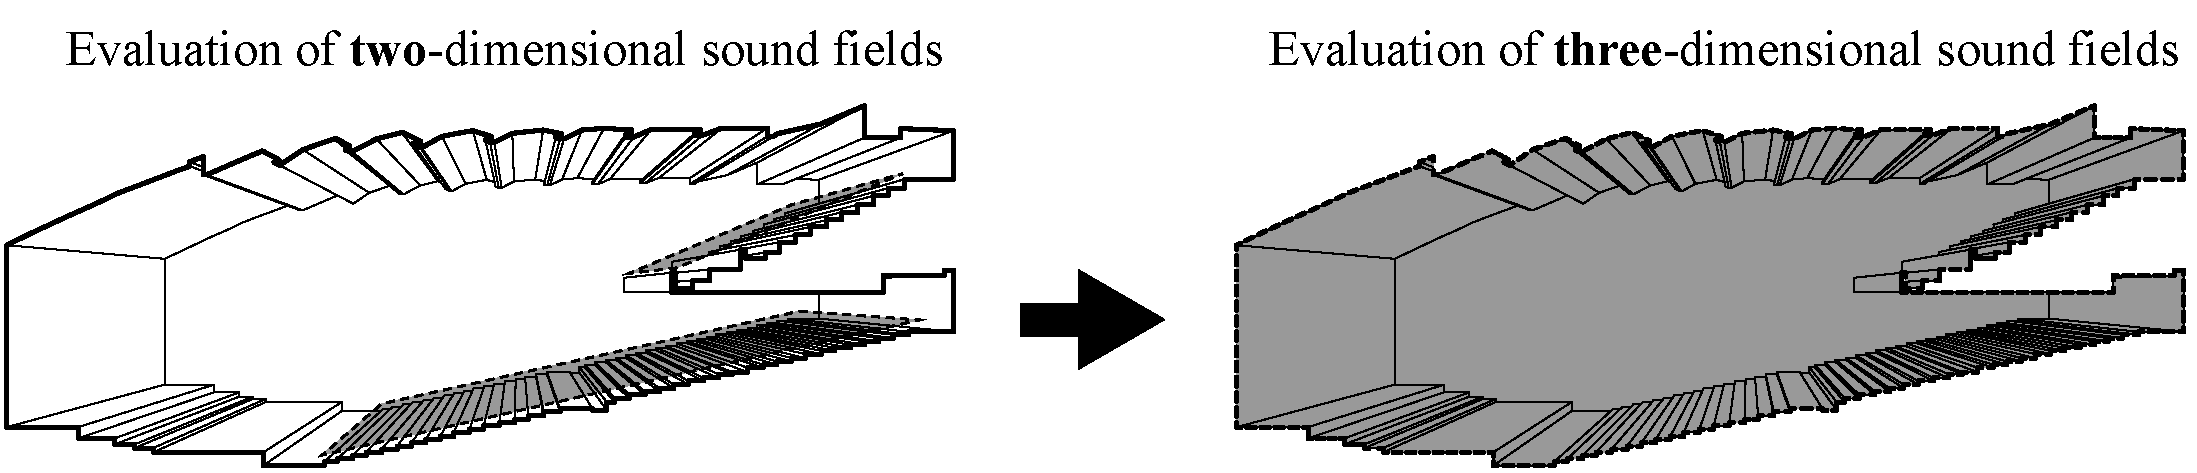
\includegraphics[keepaspectratio,scale=0.41]{01_att/evaluate_area.pdf}
    \caption{\hspace{1mm}評価対象領域の拡張}
    \label{fig:評価対象領域の拡張}
\end{figure}

\subsection{研究目的}
本研究は、コンサートホール音場の評価対象領域を、吸音力の大きな座席面近傍音場から3次元的に拡張し、座席面遠方音場(\textgt{図}\ref{fig:座席面遠方音場})の音響物理特性を明らかにすることにより、従来の面的評価並びにそれに基づく決定論的設計法に新たな可能性を見出すことを目的とするものである。
\\
\begin{figure}[h]
    \centering
    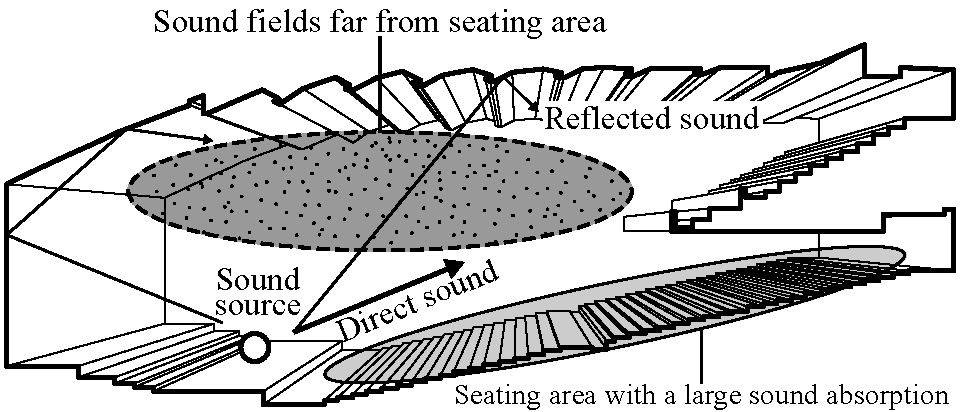
\includegraphics[keepaspectratio,scale=0.8]{01_att/zasekimen_enpo_English.pdf}
    \caption{\hspace{1mm}座席面遠方音場}
    \label{fig:座席面遠方音場}
\end{figure}

%-------------------------------------------------------------
\newpage
\section{既往の研究と本論の位置づけ}
\subsection{音環境の心理評価システム}
物理的特性と聴覚的効果との対応を考える必要があることを説明する
\\→本論文は物理的特性をとりあげた研究であること(聴覚的効果との対応は含まない)を言及する。

\subsection{室内音響物理指標}
4つの要素感覚とそれに対応すると提案されている物理量について説明する。

\subsection{フライングバルコニーを有するホールの事例}
Philharmonie de Parisを例にフライングバルコニーの紹介、本研究のテーマに近いホールがあることを示し、本テーマは突拍子もないことではないことを示す。

\section{論文構成}
本論文は、以下に示す全7章で構成される。
\\ 第1章では前節までに本研究の背景と目的、関連する既往研究の概要、本論の位置づけについて述べた。本節では、論文の構成について述べている。
\\ 第2章では、研究手法である幾何音響解析の概要、解析条件並びに解析モデルについて述べる。
\\ 第3章では、解析で得られたデータから残響特性の観点から音場評価を行う。
\\ 第4章では、時間エネルギ特性の観点から音場評価を行う。
\\ 第5章では、反射音方向分布特性の観点から距離減衰特性及び方向別エネルギ率の観点から音場評価を行う。
\\ 第6章では、これまでの研究結果を踏まえ、ホール形状の設計例を提示する。
\\ 最後の第7章では、本論文の結論を述べる。
